
\title{A Very Simple \LaTeXe{} Template}
\author{
        Vitaly Surazhsky \\
                Department of Computer Science\\
        Technion---Israel Institute of Technology\\
        Technion City, Haifa 32000, \underline{Israel}
            \and
        Yossi Gil\\
        Department of Computer Science\\
        Technion---Israel Institute of Technology\\
        Technion City, Haifa 32000, \underline{Israel}
}
\date{\today}

\documentclass[12pt, titlepage]{article}
\usepackage[utf8]{inputenc}
\usepackage[T1]{fontenc}
\usepackage{lmodern} % load a font with all the characters
\usepackage{graphicx} % includegraphics command is implemented here
\usepackage{float}
\usepackage{listings}
\usepackage{xcolor}

\colorlet{punct}{red!60!black}
\definecolor{background}{HTML}{EEEEEE}
\definecolor{delim}{RGB}{20,105,176}
\colorlet{numb}{magenta!60!black}

\lstdefinelanguage{json}{
    basicstyle=\normalfont\ttfamily,
    numbers=left,
    numberstyle=\scriptsize,
    stepnumber=1,
    numbersep=8pt,
    showstringspaces=false,
    breaklines=true,
    frame=lines,
    backgroundcolor=\color{background},
    literate=
     *{0}{{{\color{numb}0}}}{1}
      {1}{{{\color{numb}1}}}{1}
      {2}{{{\color{numb}2}}}{1}
      {3}{{{\color{numb}3}}}{1}
      {4}{{{\color{numb}4}}}{1}
      {5}{{{\color{numb}5}}}{1}
      {6}{{{\color{numb}6}}}{1}
      {7}{{{\color{numb}7}}}{1}
      {8}{{{\color{numb}8}}}{1}
      {9}{{{\color{numb}9}}}{1}
      {:}{{{\color{punct}{:}}}}{1}
      {,}{{{\color{punct}{,}}}}{1}
      {\{}{{{\color{delim}{\{}}}}{1}
      {\}}{{{\color{delim}{\}}}}}{1}
      {[}{{{\color{delim}{[}}}}{1}
      {]}{{{\color{delim}{]}}}}{1},
}

\begin{document}
\maketitle

\begin{abstract}
Cafés are the home to many interesting ideas, it also a place where people go to meet new interesting people. In this report we discuss how a café environment can be realized online. The problem faced during the project includes overseeing, how one can look around and see other groups of people talking to each other. Overhearing, how one can listen to and find inspiration from other conversations going on in the café. Mingle, how one can move between these conversations in a subtle way.

A prototype was built using WebRTC, HTML5 and Javascript in order to solve these problems. Multiple solutions for each problem, together with a 2- and 3-dimensional views are being presented. The prototype consists of a video chat with multiple extra features for collaboration, like shared napkin to paint on and  synchronized Youtube watching, implemented to enhance the feeling of sitting at the same table. 
\end{abstract}
\tableofcontents
\section{Introduction}
A café is a very stimulating environment to many people. It’s a place where you can easily meet other interesting people. A place where you can walk by a table, overhear a conversation and oversee the whole café. We have all seen the group of girls sitting at a table drinking coffee and having conversations about anything, or the writer who finds inspiration for his next book from the environment and people around himself. Another scenario is all the people travelling to conferences each year. Businesses could save a lot of money if there existed a stimulating environment where one can meet people, collaborate in groups and mingle just like in the real world.

We want to transfer this feeling of being in a real café online. With the ability of seeing each other through video conference, collaborate together on a drawing, watch youtube videos, reading pdfs together and of course being able to communicate through a text chat with all the participants sitting down at a table. Three other important aspects of transferring this feeling is overseeing, overhearing and mingling. These parts will be investigated and tested with a prototype.

When you are walking by a table in a real café you will hear what their conversation is about and also see all the participants, this is overhearing and overseeing. Before you can sit down at a table and join a conversation you will gently ask if it is okay without trying to disturb their conversation too much.

The prototype contains a 2D- and 3D-view where overseeing, overhearing and mingling is realized.

\subsection{Problem description}
The problem we set out to solve was how to create a web based environment for sharing the feeling of being in a Paris Café including how to convey a feeling of overseeing, overhearing and mingling. Unlike traditional video chats where there is only one group of people participating, we want to create a video chat service with multiple rooms and multiple groups in each room. Where users can see the other groups and overhear conversations and move between the tables in an easy way.

Also how we can realize this feeling in a 2 and 3 dimensional view and still keep the café feeling, low latency so it feels like a “real” meeting, video streams instead of avatars and present them in a nice way in both views.
\subsection{Project goals}
The goal of the project is to:
\begin{itemize}
  \item Create a working prototype
  \item Implement some kind of overhearing
  \item Implement some kind of overseeing
  \item Implement some kind of mingle
  \item 2D and 3D view
  \item Evaluate the system with a user test
\end{itemize}
Implementing some kind of overhearing, overseeing and mingle is vague but here are some ideas for how it can be done.
\subsubsection{Overseeing}
How can one see the other participants at the same table while at the same time also see other groups of visitors in the same café. This could be realized with a 3D-environment with videos organized around different tables.
\subsubsection{Overhearing}
How can one hear the conversations from the other groups sitting at another table or just walking by that table. This could be realized with spatial sound in a 3D environment or by hover the mouse over a table in a 2D view.
\subsubsection{Mingle}
How can participants easily move between different conversations? I.e. if I oversee and overhear another interesting conversation, how can I gently move into that without too much interruption? This can be done by, for example, knocking, avatar gestures in a 3D world or writing a message to the group.

\subsection{Project requirements}
The project had a few restrictions of what technologies to use, WebRTC for media and data communication between clients, javascript and HTML5 for frontend. At the moment WebRTC is still under development. These technologies is used to promote using native browsers without any plugins.
\subsection{Project delimitations}
This is a big project and it need some limitations, it is our imagination and time that decides. We decided to limit us to have six cafés, six tables in each café and six persons at each table maximum. The server we are using have limitations and therefore the amount of people at each table is limited.
\subsection{Research questions}
Imagine a café in Paris where people come and sit down for a coffee and conversation. Around them other things will happen; they will see people, they will overhear conversations, they might meet old friends and engage in conversation with them for a short while. This can be done online with video chat, text chat, view videos and draw together for example on a napkin as you might do in a real café. Good video quality is needed and the fewer steps from the index-page to the actual conversation is better, due to the simplicity for the user and therefore easier to make the users experience as good as possible and hopefully they will come back.

As a part of the research, the prototype will be tested in both 2D- and 3D-view to discover which of them that achieves the most realistic way of presenting a café in Paris online.
\subsection{Related work}
Online group collaboration is an area that has been investigated and researched for many years and a number of different tools have been made available, both from research and from commercial entities. However, in a video chat, the focus has mostly been in one group chat and not to have several groups in one chat room that allows overhearing and overseeing and an easy way to move between these groups.

Video conferencing tools comes in many forms. Some are web-based like Google Hangout[6], other require software clients, like Skype[10]. Some uses avatars in a virtual environments or a mixed reality.
\subsubsection{Traditional video conference}
There are tons of group video conferencing services out on the market today. In services such as Google Hangout[6] or ooVoo[7], users transmit video and audio to each other using normal video cameras or web cameras and microphones.
\subsubsection{3D Virtual environments}
In 3D virtual environment you can create an avatar and walk around in a world with other avatars. Depending on the service you might be able to talk using spatial voice chat, text chat, mingle with other participants or explore the world together. An example of this is Second Life[3].

The key difference from traditional video conference is that you can’t see the faces of the other participants, you can only see their avatars. This can affect the social trust between participants but a study showed that participants get a feeling of being ‘there’ that traditional video conference does not support[1].
\subsubsection{Mixed reality}
Mixed reality means merging a real world with a virtual world to produce a new world where physical and virtual objects co-exists. Usage of this mixed reality has been done in order to enable human expressions and gestures on avatars in 3D virtual environment[9].
\subsubsection{Criteria}
The criteria for the comparison of the different services are based on three things. What we feel are important aspects of a real life café, what features we would like to see in an online café and the key features of the services in question.
\begin{itemize}
\item Video chat - If it has video chat or not
\item Free - If it’s free or paid
\item Record - If it’s possible to record your chats
\item Share screen - If it’s possible to share your screen with other participants
\item Broadcast - If it’s possible to broadcast your video
\item Collaboration - If it’s possible to ex. write documents or view presentations together
\item Requires software - If there is a client that needs to be installed
\item Mobile version - If there is a mobile version of the service
\item File transfer - If it’s possible to share files
\item overhearing - If it’s possible to overhear conversations of other people using the same service.
\item overseeing - If it’s possible to oversee other people using the same service
\item mingling - If it’s possible to easily join a conversation without too much disturbance.
\end{itemize}
\subsection{Related services}
Here follow some information about each service and what makes them unique. Each service is compared to the list of criterias.
\subsection{Google WebRTC}
WebRTC is a new open-source project which aims to enable real-time communication(RTC) in web browsers with simple Javascript APIs. It’s currently under development but Google Chrome and Mozilla Firefox have recently managed to communicate between the browsers[13].
\subsubsection{Browser meeting}
Browser meeting[12] is a web application using WebRTC. It’s a web conference tool which is very easy to use. Simply create a room and invite your friends.
\subsubsection{frisB}
FrisB[15] is a web based application and a voice channel that freely 'ring invites' any telephone user on the planet into a conversation. No video or text chat is offered. This application uses WebRTC.
\subsubsection{Video Conference in 3D Environment}
By using both WebRTC and WebGL you can for example video chat with your friends in a virtual 3D environment. One application, WebGL Meeting[18], let you chat in real-time with the people you invite to your room that automatically creates when you enter the website.
\subsection{Protonsphere}
Protosphere is a secure private 3D virtual environment where you control an avatar in order to collaborate and socialise with other participants.
\subsection{O.L.I.V.E}
SAIC O.L.I.V.E[4] is an online Interactive virtual environment software platform that delivers interactive multimedia communication capabilities for collaboration, training, operations and education. It is possible to video and text chat through an avatar with voice, you can also record the conversations. During training and education with O.L.I.V.E broadcasts and collaboration is used. You are able see, hear and mingle with the other participants.
\subsection{OpenQwaq}
OpenQwaq is an open source software which aims to allow businesses to implement their own virtual world workspaces adjusted for their specific needs. It provides all the tools, data, and interactivity that people need to explore ideas, resolve issues, track progress, and be more productive.
\subsection{Paltalk}
Paltalk is an instant messaging service which allows users to communicate via text, voice and video chat. It lets users create their own public chat rooms where they can talk with their friends or find new ones. Paltalk exists in three different forms. Paltalk messenger which is a downloadable client, Paltalk Mobile, the phone version and Paltalk Express, a web version.
\subsection{Tiny Chat}
TinyChat is a small simple video chat. Create a chat room, invite your friends or make new ones. An interesting part of TinyChat is their API which allows you to implement your own fully functional chat room wherever you want. Other features are screen sharing, broadcast and more.
\subsection{Skype}
Skype is a service which aims to make it easy to stay in touch. It does this by enabling free internet calls, instant messages and video chat. What makes Skype special is the ability to buy Skype Credit for which you can make cheap calls to phones and mobiles, get online at public WiFi hotspots and send SMS worldwide. Skype require a client and has a mobile version.
\subsection{Google Hangout}
Google hangout[6] allows you to video chat with up to 9 other people in a hangout. One cool thing with Google hangout is that it has apps, for example YouTube, Poker, and Google Docs. These makes it possible to for example, watch videos together or view presentations and diagrams with your co-workers. You can also broadcast your hangout with Hangout on air. Everything you broadcast is recorded and stored on your YouTube channel.
\subsection{ooVoo}
OoVoo[7] is another interesting video chatting system. In contrast to Google hangout, ooVoo requires a client to be installed. Once installed you can video chat with up to 11 other people, send video messages and text chat. The video chatting can be recorded and uploaded to youtube.
\subsection{Second Life}
Second Life[3] is a 3D virtual environment where everyone you see is a real person and every place you visit is built by people in the virtual world. Setup and design your own 3D-avatar to join a 3D world. After downloading and installing the client you can start text chat with other people online in the world that you see. It exists different types of room you can visit, for example a night club, beach or London city town. There exists both paid and free versions. Some of the rooms also have voice chat to offer their visitors.
\subsection{The Word Cafe online community}
The world cafe online community[8] is a website who offers a place online to have great and meaningful conversations about things you care to discuss about. There is no video chat or sharing media with each other, only text chat, more like a forum. Everybody gets their own blog to share their interest with everybody and start a conversation. The site is free to use, they offer their users to take online courses, some of them are free. The courses are held at the site. It exists a mobile page for your mobile phone or tablet. When register you have to be approved by the administrators before you become a “real” user.

\subsection{Related papers}
Online video collaboration has been researched for a long time by many different teams. There exists a large number of solutions for video conferencing systems each using different technologies to solve their specific problems. Back in 1995 some researchers in Japan created a video conferencing system called MAJIC[17]. It was a multi participant system that enabled eye-contact with life-sized images of each other. It also had a shared workspace which enhances the collaboration. Evaluation of the system showed that the background influences the sense of presence and that life-sized images gave a sense of reality.

The MAJIC system was fairly big due to the life-sized images and eye-contact solution. Some other researchers proposed a solution for eye-contact using a single Kinect sensor[21]. They do this by rendering a gaze-corrected 3D model of the scene and transfer the gaze-corrected facial portion onto the original image using a face- tracker. The result was fairly good.

Another gaze correction study is done to establish if it is possible to do this correction even with movement during a video conference[20]. The paper aims to show that, while both integrating eye-trackers into an Immersive collaborative virtual
environments (ICVE) and video conference, allow people to distinguish being looked at and what else is looked at, when someone gazes into their space from another location, ICVE alone can continue to do this as people move. The result shows that only the ICVE supports eye gaze correction movement of the observer.

Other researchers tried to improve this feeling of presence and realism by using a movable camera[19]. The system has a remote camera which moves forward when a local user approaches the screen. This gives both users a good perspective when looking at the other person during a video chat. It gives the feeling of facing a remote person in the same room.

Microsoft researchers tried a different solution. Instead of using hardware they came up with a software solution[22]. They tracked the participants head and eye movements and used this information to place the head and eyes in a 3D environment. Although the resulting system was kind of slow, it showed that it is definitely possible to do with only software.

Group video conferencing requires some hardware and bandwidth in order to transfer the audio and video between all the participants.
One paper proposed an architecture for a peer-to-peer multipoint video conferencing system with layered video aimed for end-points with low bandwidth[14]. The system enables the participants to create a group conference using no more bandwidth than a point-to-point system. A prototype is created and the system is validated.

DigiMetro[16] is a proposed design for an application-level multicast system for a small-scale video conferencing tool. It takes use of multiple source-specific trees in order to keep the delay down. DigiMetro allows different bit-rates on different sources which makes it possible to use even with low bandwidth.

Many solutions by, for example Cisco and HP, require a large stationary and expensive setup in order to work and does not even then solve the problems good enough to give the feeling of sitting in the same room. The European FP7 project 3DPresence[23] came up with a concept for a high-end 3D Video conferencing system that aims to solve several of the problems that comes with video conferencing, including life sized participants, mutual gaze and gesture awareness.

In contrast, TAM TAM[24] minimalistic video conferencing system designed for the browser and mobile devices. It is built using Adobe Flash and Adobe Air, which makes it possible to run on platforms such as Windows, Android and iOS.

Online mingle and overhearing have received little attention from researchers. One of the few services which allows mingling is Second Life[3]. An evaluation of a big conference in Second Life done by IBM[1] showed that although the avatars helped created a feeling of being there[11], the sound of people talking travelled too far. This meant groups of people had to walk far away from each other or end up interrupting another or multiple other conversations. Some also said that it was hard to know if it’s okay to join a conversation or not due to the lack of human expressions and gestures. An advantage of online mingling is that each avatar may have a name over his head which makes it easy to recognize acquaintances. A disadvantage however is that it does not feel as personal as if you had met face to face[1].

Overseeing in 3D worlds already exists[2][3][4][5], in a 2D world this can not be realized in the same way as i in a 3D world. That will be a part of our master thesis to discover if there is a way to realize it.
\subsection{Project transparency}
One thing that our supervisor, Peter Parnes usually requests in all his courses is that the progress of the project should be periodically updated in blog posts. The idea is that everyone should understand the posts and it makes it easy for us to see what problems we run into during the project.

Before this project started we made a gantt-chart, a rough plan of our milestones of all 20 weeks. The first five weeks was dedicated to competitive intelligence, research what technologies that is suitable for our prototype and feature planning. The next 12 weeks were spent implementing the prototype, bugfix, find improvements and writing report. We had to make some small adjustments to the 3D-view, and delimit some features due to the lack of time. The last three weeks was used to fix some bugs, writing report and the final presentation.
\begin{figure}[h!]
  \centering
	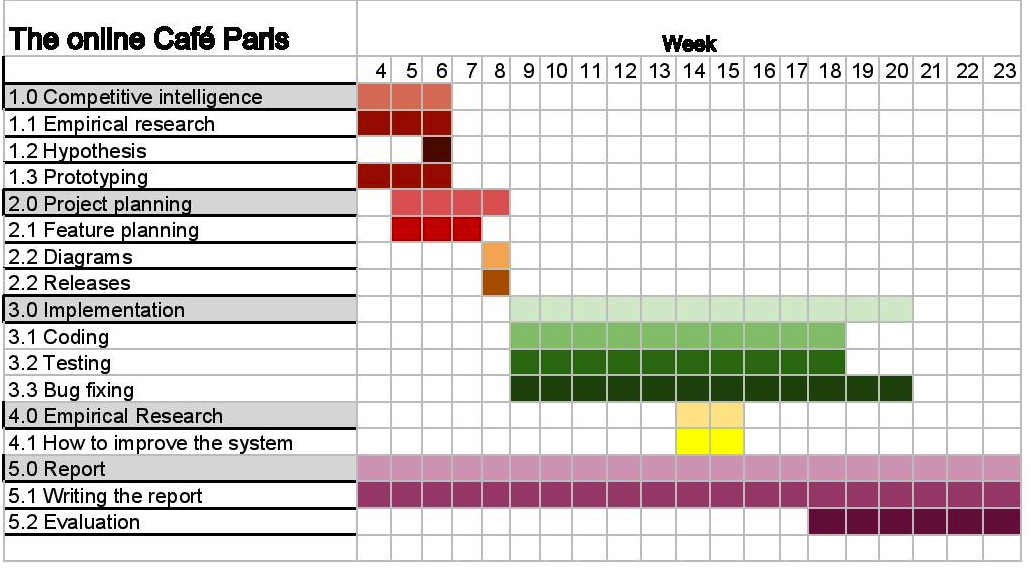
\includegraphics[width=0.8\textwidth,keepaspectratio]{grovplanering.jpg}
  \caption{A gantt-chart to guide us through the project and manage deadlines.}
\end{figure}
The work has been shared equally between the two participants in this project. All the planning, prestudy and implementing of the prototype was done together.
\subsection{What the site looks like}
These pictures will give you an idea of how the site is build up and it is easier to understand the idea, technologies, features and of course the design.
\subsubsection{Index/start page}
\begin{figure}[H]
  \centering
	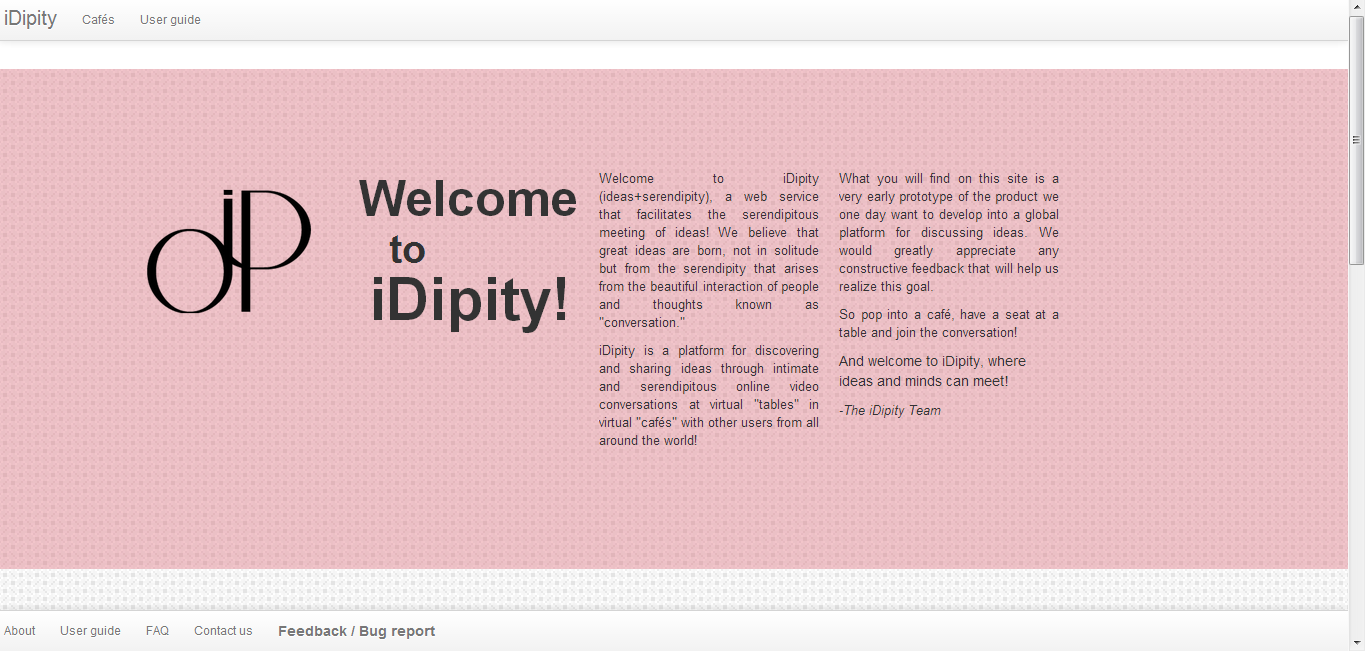
\includegraphics[width=0.8\textwidth,keepaspectratio]{indexpage1.png}
  \caption{The start page with a welcome message and some information about the site.}
\end{figure}
\begin{figure}[H]
  \centering
	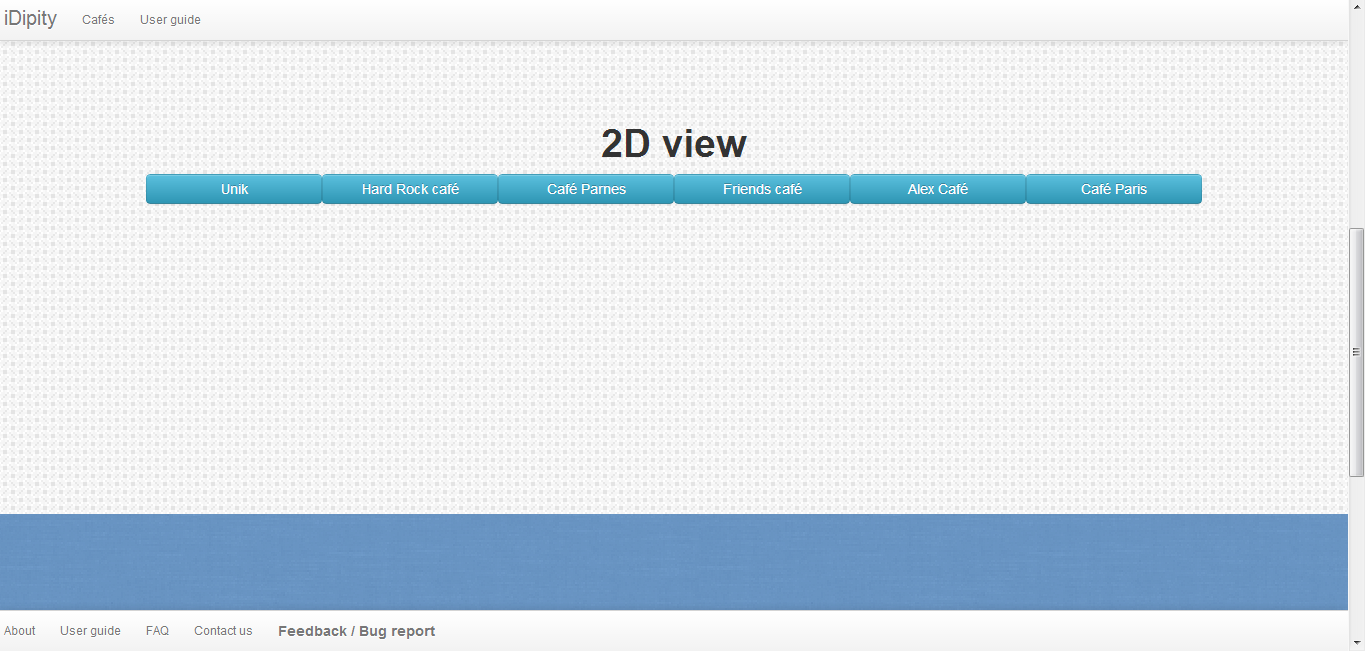
\includegraphics[width=0.8\textwidth,keepaspectratio]{indexpage2.png}
  \caption{The start page, the buttons are the six cafés the user can visit, this is the 2D view.}
\end{figure}
\begin{figure}[H]
  \centering
	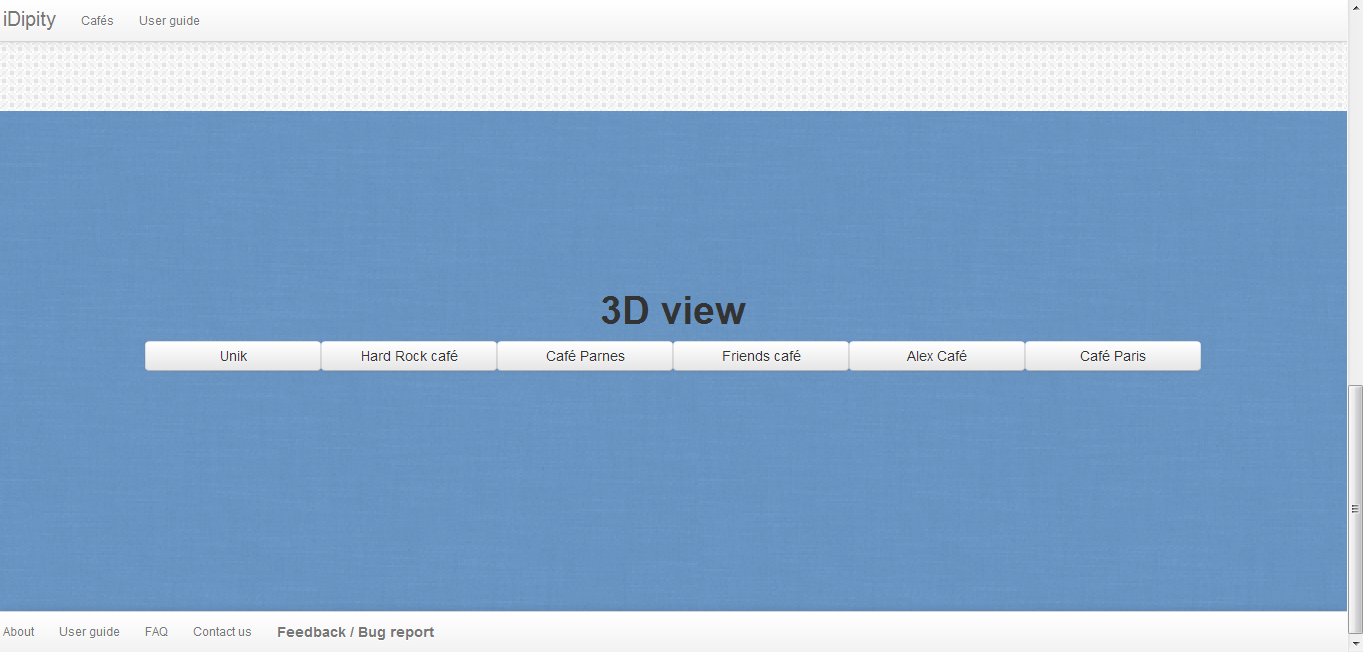
\includegraphics[width=0.8\textwidth,keepaspectratio]{indexpage3.png}
  \caption{The start page, the buttons are the six cafés the user can visit, this is the 3D view.}
\end{figure}
\subsubsection{Cafeview}
\begin{figure}[H]
  \centering
	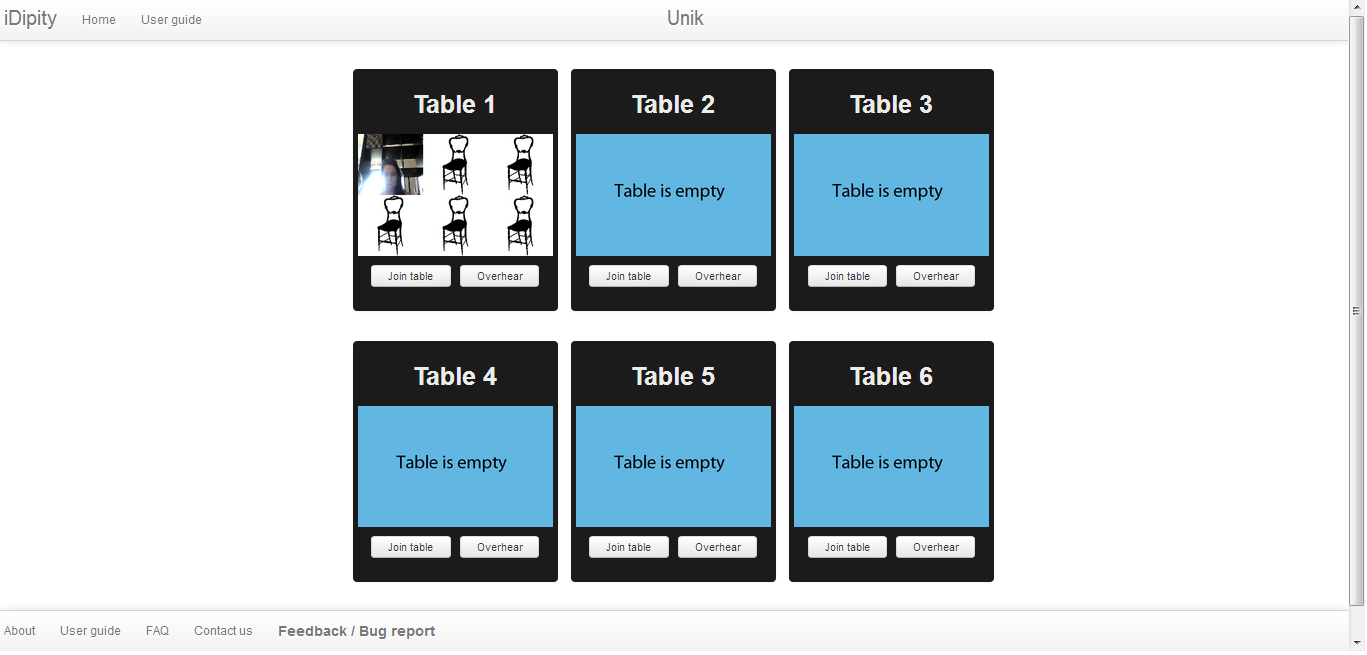
\includegraphics[width=0.8\textwidth,keepaspectratio]{thetables.png}
  \caption{This picture shows the tables in the café Unik. In table 1 there is one person sitting down, the other seats is empty at that table.}
\end{figure}
\begin{figure}[H]
  \centering
	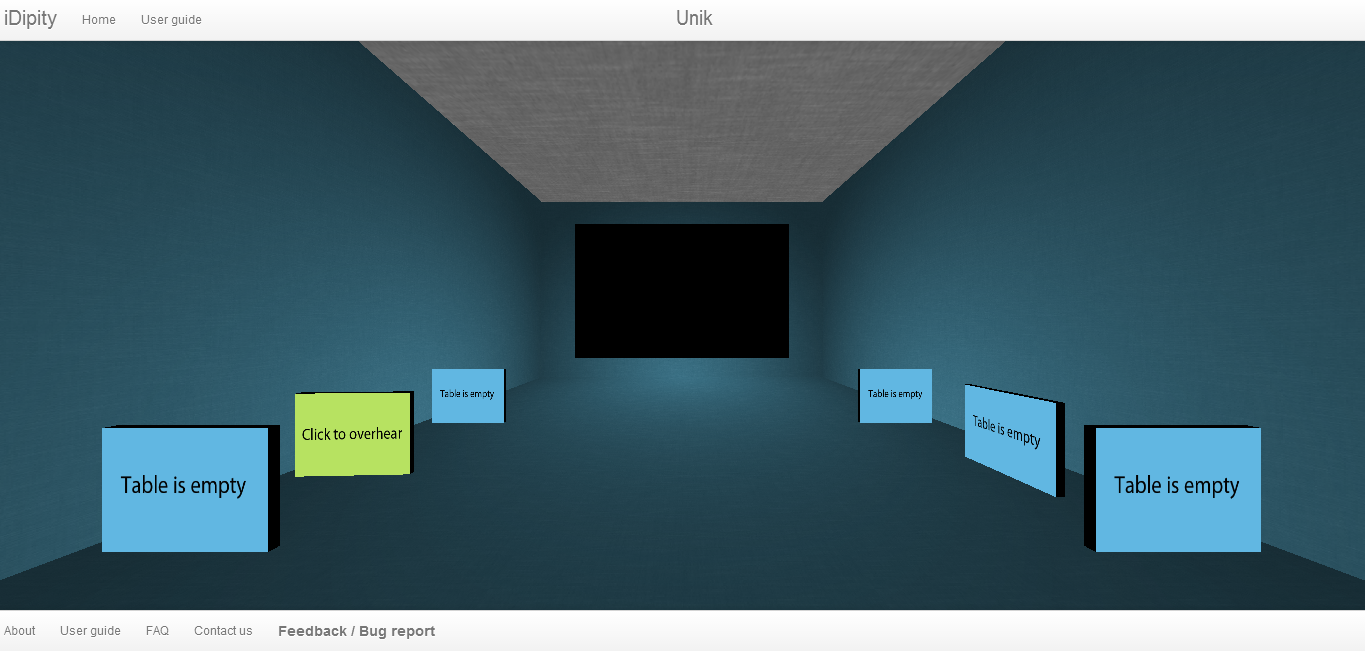
\includegraphics[width=0.8\textwidth,keepaspectratio]{thetables3D.png}
  \caption{This picture shows all the tables in café Unik. At the moment all the tables are empty. The green table is turned around with the mouse, if you click the on the turned table you will overhear the conversation if the table is not empty. If you click at a table you will sit down at the table.}
\end{figure}

\subsubsection{Tableview}
\begin{figure}[H]
  \centering
	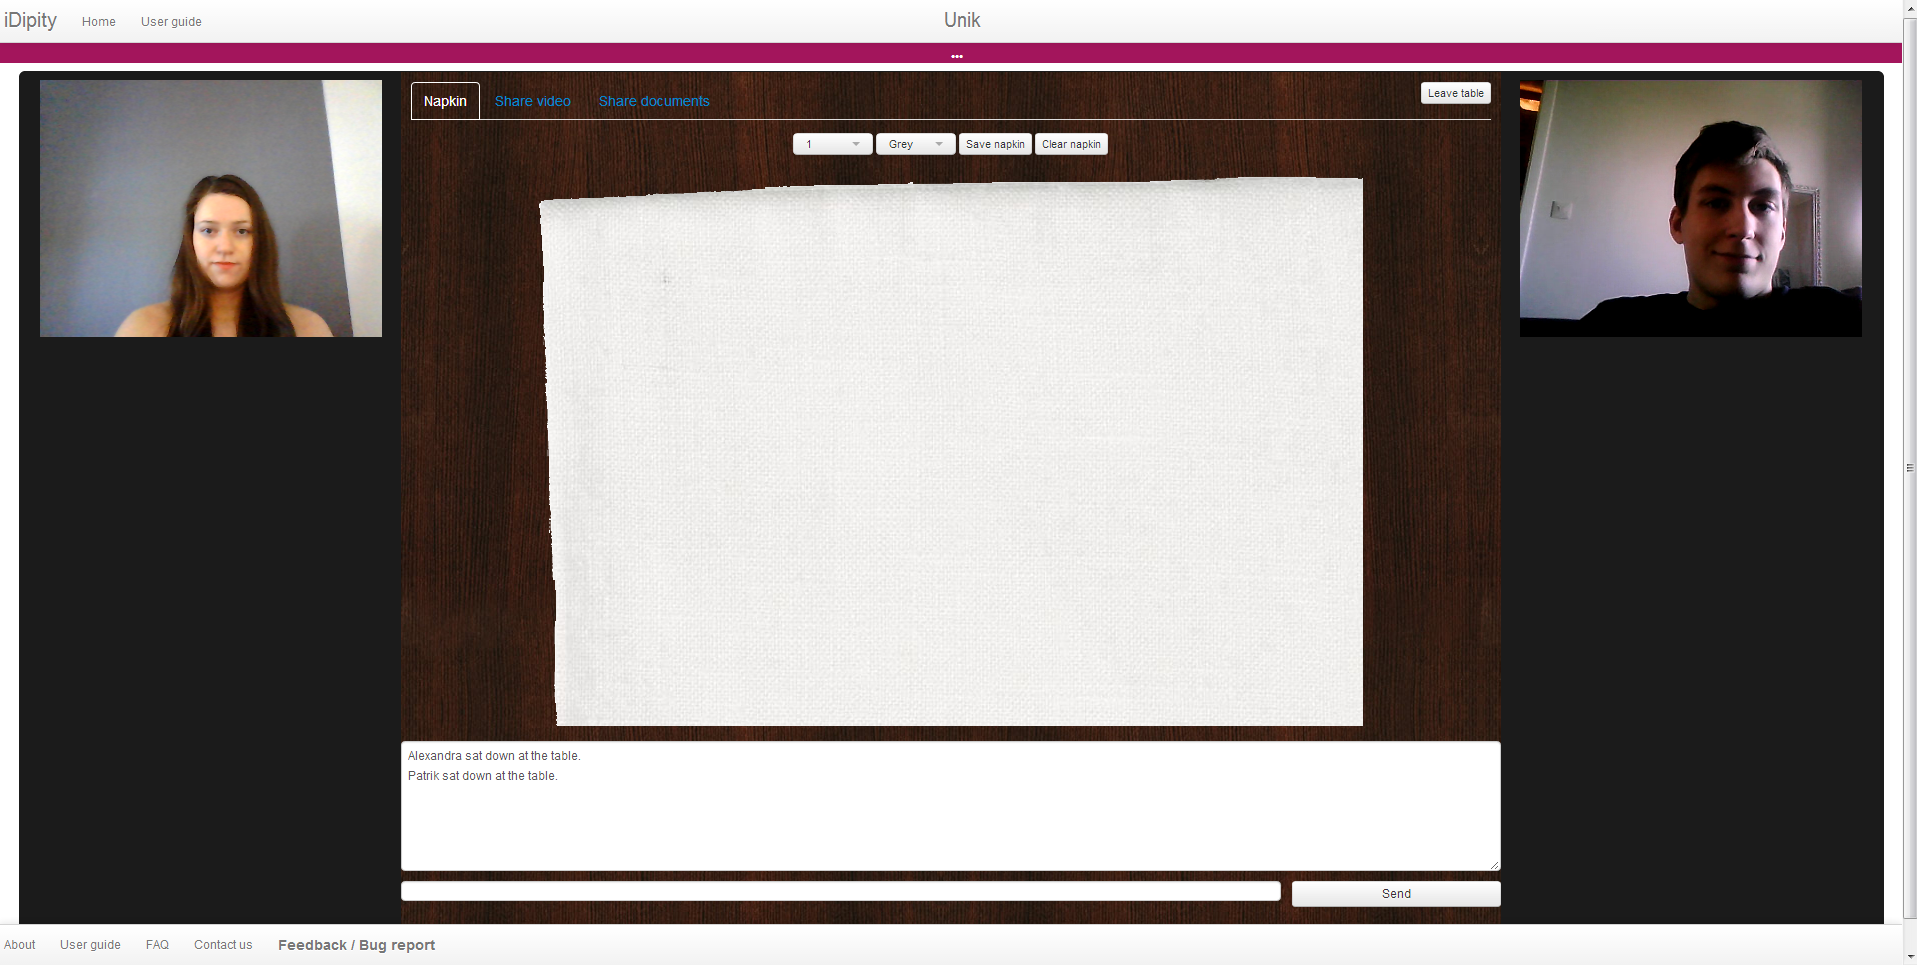
\includegraphics[width=0.8\textwidth,keepaspectratio]{sittingdown2D.png}
  \caption{This is how it looks like when you sitting down at a table having a video conversation with someone. You see the text chat and the napkin.}
\end{figure}
\begin{figure}[H]
  \centering
	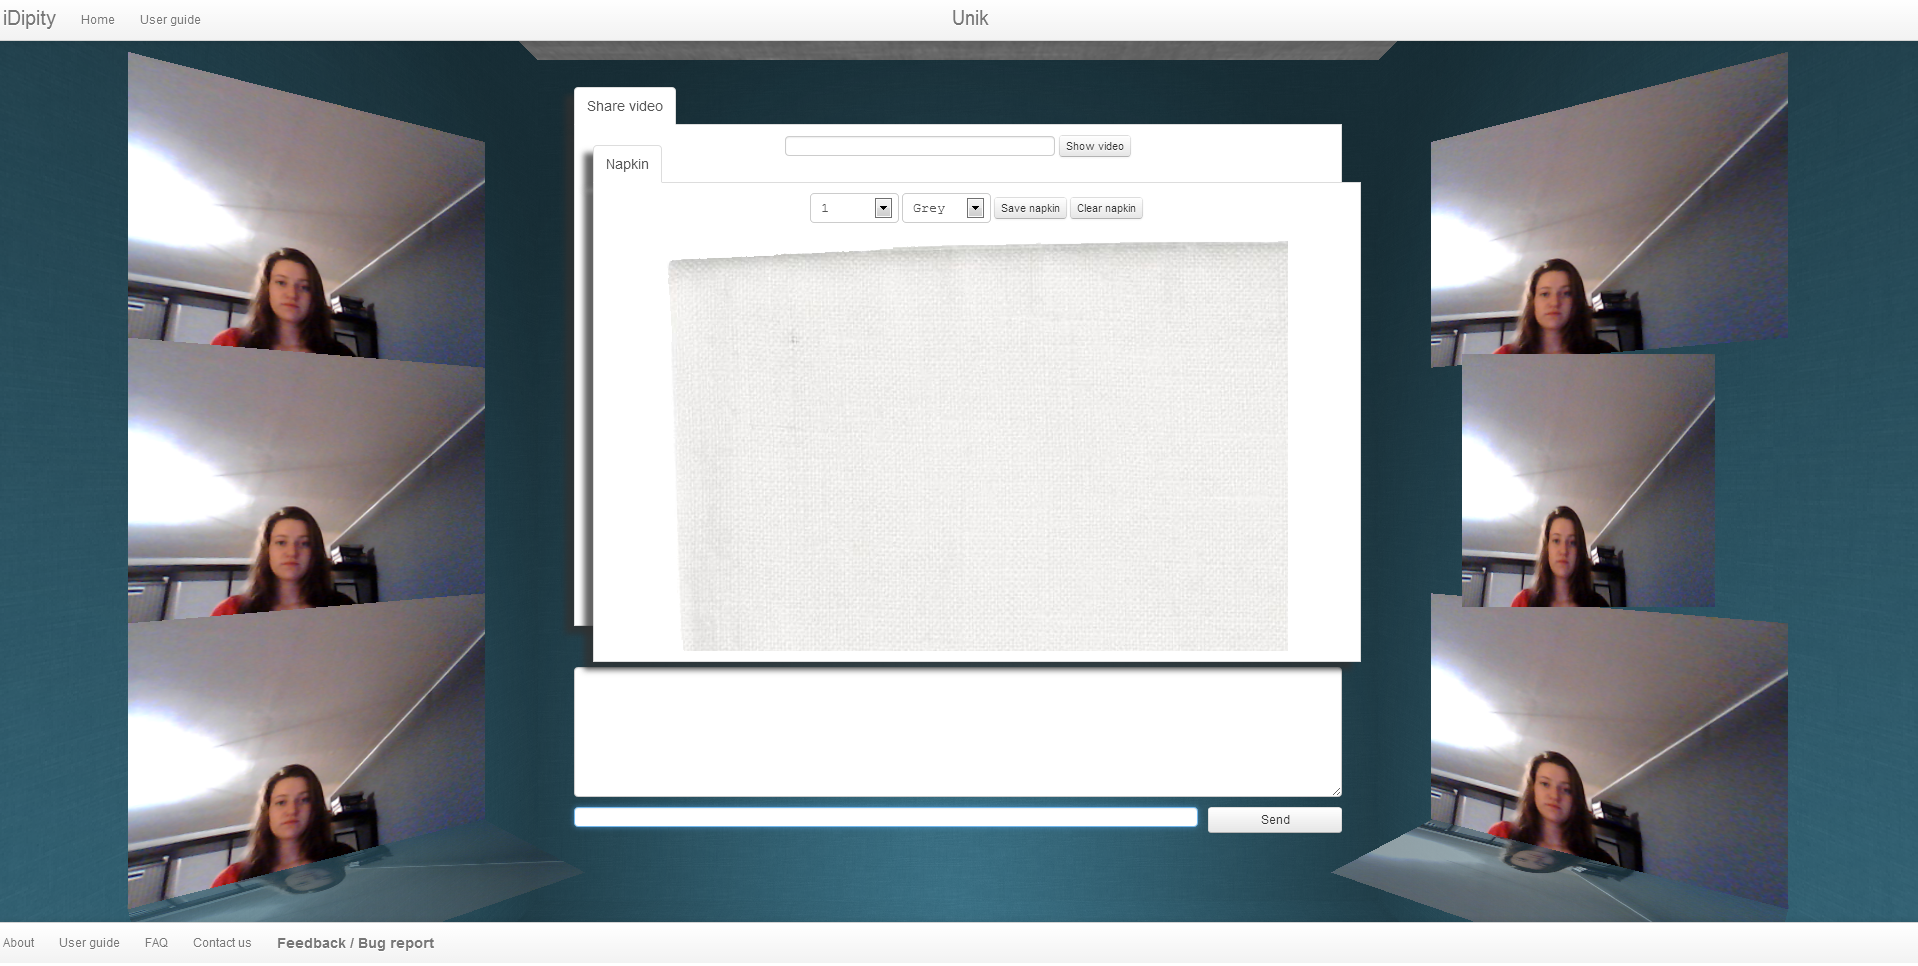
\includegraphics[width=0.8\textwidth,keepaspectratio]{sittingdown3D.png}
  \caption{This is how it looks like when you sitting down at a table having a video conversation with someone. You see the text chat and the napkin. The video stream in middle to the right has a mouse over it. That is why it looks different.}
\end{figure}
\subsection{Use cases}
These use cases are made for a better understanding of how the system can be used. Three example will explain this.
\subsubsection{Use case 1: Enter a café}
Lisa has a new idea for a product she wants to discuss. She starts her web browser and open Paris Café web page. She is met with a welcoming message and a list of the available cafés. After choosing a café she will be asked to enter her name into a form before continuing to the tables of the café. Once done she will be met by six “tables”. 
\subsubsection{Use case 2: Oversee and overhear}
When Lisa is inside a café she can look at the six tables. Each table will display an image of the persons, if any, sitting at the tables. When she has found a table that looks interesting she can choose to overhear and oversee the persons at the table by clicking the button “overhear”. The image will then be replaced by live video streams of the participants, including audio.
\subsubsection{Use case 3: Sit down at table}
After finding a table to sit down at she clicks “Join table”. Participants of the group will hear a knocking sound and find a notification in the upper right corner. They will now answer yes or no. If the majority answer yes she will sit down at a table where the video chat begins.
\section{Technologies}
\subsection{Node.js}
Node.js is an event-driven, non-blocking I/O JavaScript platform, built on Chrome’s V8 JavaScript runtime. The reason for using Node.js is that it makes for easily building fast and scalable network applications. The server is entirely written under the Node.js platform.
\subsection{WebRTC}
WebRTC (Web Real-Time Communication) enable browser to browser applications for voice calling, video chat and peer-to-peer file sharing without any plugins. A requirement for WebRTC is to use it in conjunction with HTML5. WebRTC is available in Chrome's stable version and in Firefox's Nightly version.

By using peer-to-peer connection instead of sending information through a central server, it removes the need for a powerful server. A server is still needed to setup the connection between the participants.
\subsection{Licode}
Licode is an open-source project that is based upon WebRTC technologies. It comes with Erizo, a Multipoint Control Unit(MCU) and an easy to use API for creating video conference rooms directly in the browser. 
\subsubsection{Erizo}
Erizo is an MCU written in C++. It’s fully compatible with WebRTC standards and protocols. Erizo does not currently provide any transcoding of videos but it’s being worked on right now. 
\subsubsection{Nuve}
Nuve makes it possible to create and manage video conference rooms. It holds information about each room and let’s you ask for example a user list. It is designed to scale on the cloud.
\subsection{MongoDB}
MongoDB is an open-source, document-oriented database designed for ease of development and scaling. Stores data as JSON-like documents dynamically and making the integration of data and our prototype easier and faster.
\subsection{Mongoose}
Mongoose is an object data modeling library for MongoDB. It allows you to create models for your data, creating a structure to MongoDB while maintaining it’s flexibility.
\subsection{Express js}
Express is a fast and small node.js web application framework, providing a powerful routing system which allows you to easily create single and multi-page web applications. It helps you manage everything, from routes, to handling requests and views.
\subsection{Twitter Bootstrap}
Twitter Bootstrap is a collection of tools for creating beautiful web applications without being an expert on design. It includes HTML, JS and CSS-based design templates for typography, forms, buttons, charts, navigation and other interface components. The reason for using Twitter Bootstrap is to get a nice interface and it is easy to use.
\subsection{HTML5}
HTML is used to structure and presents information on a website, HTML5 is the newest HTML standard. It’s designed to make web programming easier and more interactive. Some of the new features that are interesting for our project is the <video> and <canvas> elements.
\subsection{Three.js}
Three.js is a lightweight cross-browser JavaScript library/API used to create and display animated 3D computer graphics on a Web browser. Three.js scripts may be used in conjunction with the HTML5 canvas element, SVG or WebGL. We decided to go with WebGL.
\subsubsection{WebGL}
WebGL (Web Graphics Library) is a JavaScript API that allows the client to render powerful 3D graphics within the browser without plugins. It runs on computers GPU.

Our purpose of using WebGL is to try the café Paris website with a virtual 3D environment. This makes us a good case to try out a mixed reality, by combining a virtual 3D environment with the users video stream we can transfer the feeling of actually being in a real café into our website. Overseeing, overhearing and mingling
\subsection{Github}
For revision control and code management we use Git. Git is a open source distributed revision control system. To simplify the setup we chose to host the repository at Github.


\section{Method}
Some information was collected before implementing the service. A study was made in order to find suitable ways of overhearing, overseeing and mingle. And a comparison of different WebRTC frameworks was necessary for us due to the video conference features.
\subsection{WebRTC comparison
WebRTC is a new web standard for peer-to-peer communication. WebRTC allow browsers to send information to each other, without going through a server. The focus is currently on audio and video communication but they will implement a data channel in the future. This will drastically decrease the server load.

We compared many different WebRTC framework before settling with Licode. Licode offered something that others didn’t, and something that is necessary if the system would be used on a larger scale. That feature is a Multipoint Control Unit(MCU). Here follows a short summary of the runner ups.
\subsubsection{Easy RTC}
EasyRTC is an open source WebRTC framework with cross browser support. It allows you to easily steup a Node.js server and provides an API for making advanced web applications in no time. EasyRTC uses websockets for fast message passing between clients.
\subsubsection{WebRTC.io}
WebRTC.io aims to make it easier to use the new webstandard. It does this by providing a simple abstraction layer for the otherwise semi-low level WebRTC.
\subsubsection{Holla}
Holla is another abstraction layer with the same goal, to make it easier to work with WebRTC. Holla provides a client and a Node.js server module. The server is used to initiate the communication between the clients. Each client registers a username that is used for making calls or sending data to each other.
\subsection{Survey}
A survey was made during the early stages of the project. The idea was to get a grasp of how people feel about visiting a virtual café online as well as to capture their opinion on what aspects of a real café makes it such a good place for intimate discussions.
\subsubsection{Evaluation}
The most important aspects of a café is the intimate environment and the other people in the café. This means that in order for us to capture that intimate feeling of a café, we have to create a design that gives a similar feeling

The result showed that people like the ability to overhear other conversations going on in the café. But it also showed that it can be a disturbing factor when you can’t block out the noise.

Mingle is big part of the master thesis. How can you ask to participate in a conversation without disturbing the group of people having the conversation. The answers shows that a subtle knock or a short personal message to the group would get their attention without drawing them away from the conversation.

We had a few questions concerning a 3D environment. The answers however were pretty much evenly distributed between “yes” and “no” and due to the amount of participants we can’t see any clear result. However, we believe that it can be hard to imagine going to a café in a 3D virtual environment and that a new survey when we have a prototype running would result in different answers.
\subsection{Prestudy conclusion}
After doing this research we have noticed the huge amount of different video conferencing systems each with their own solution for specific problems. All from high-end systems designed for big businesses, to small systems for personal use.

The result however, strongly motivates our research questions. While there exists a few good services for video conference and online group collaboration the only ones that support multiple groups is within a 3D environment and not one of these have strong focus on mingling.

There is still room for improvements in overhearing and mingling, both inside and outside a 3D environment.

If using virtual 3D environments, a mixed reality is interesting for us to mix real peoples video stream with an virtual environment. If a person who has joined a conversation at a table does not want to share his video stream he may just get an avatar to represent him instead a video stream. It would also make it possible to enable human expressions and gestures[9].
\section{Previous work}\label{previous work}
A much longer \LaTeXe{} example was written by Gil~\cite{Gil:02}.

\section{Results}\label{results}
In this section we describe the results.

\section{Conclusions}\label{conclusions}
We worked hard, and achieved very little.

\bibliographystyle{abbrv}
\bibliography{simple}

\end{document}
This is never printed
